% Set the author and title of the compiled pdf
\hypersetup{
	pdftitle = {\Title},
	pdfauthor = {\Author}
}

\section{Distributed computing}
% Lecture One

A distributed system is a computing platform build with many computers that:

\begin{itemize}
  \item Operate concurrently,
  \item Are physically distributed (and can fail independently)
  \item Are linked by a network
  \item Have independent clocks
\end{itemize}

Leslie Lamport once said that:

\begin{aquote}{Leslie Lamport}
You know you have a distributed system when the crash of a computer you’ve never
heard of stops you from getting any work done.
\end{aquote}

The consequences of having a distributed system is that many problems can arise
from a lack of synchronization and coordination between parts of the system.
Problems include:

\begin{itemize}
  \item Non-determinism
  \item Race conditions
  \item Deadlocks and synchronization
  \item No notion of a correct time (no global clock)
  \item No (visible) global state
  \item Parts of the system may fail independently
\end{itemize}

Despite these problems, we continue to (and increasingly commonly) build systems
and software designed to run on distributed hardware. This is for many reasons,
including the fact that people are distributed and move around a lot, information
needs to be shared, hardware can be shared to reduce costs or work in parallel
etc.

Distributed systems have evolved from simple systems in the 70's and 80's. Early
systems were for banks and airline booking systems, but the real proliferation
of the technique arose with the internet in the early 90's.

There are eight so called \textit{fallacies} of distributed computing:

\begin{enumerate}
  \item \textbf{The network is reliable}\\
    The network could stop working at any time for a variety of reasons;
    hardware failure, malicious actors etc. In order to protect against this, we
    need to build clever software that can resend failed messages, reorder
    messages, verify the integrity of messages etc.
  \item \textbf{Latency is zero}\\
    Latency is the time it takes from a message to get from one place to
    another. Even if the data is going at the speed of light, then a packet
    going from London to the east coast of the USA will take $30 milliseconds$.
    Developers should make as few calls to networked machines as possible, and
    transfer as much data as possible each time.
  \item \textbf{Bandwidth is infinite}\\
    Bandwidth is how much data you can send in a certain amount of time, and is
    measured in bits per second. Bandwidth is growing as technology improves,
    but so do the data requirements of applications, meaning that it is still an
    issue. Lost packets can reduce bandwidth, so increasing packet size can
    help. Compression can also be of use.
  \item \textbf{The network is secure}\\
    Since networks are largely insecure, you need to think about application
    security all the time. Implementing access control etc is a good idea for
    networked applications.
  \item \textbf{The network topology doesn't change}\\
    Since we don't control the network, servers could be added or removed,
    clients can change addresses etc and we won't know in advance. Distributed
    applications must be adaptive and work around these unexpected changes. The
    DNS system is a good example.
  \item \textbf{There is one administrator}\\
    Different people are in charge of different networks, even different parts 
    of networks. Diagnosing a problem may require the help (and cooperation) of
    multiple people and organisations.
  \item \textbf{Transport cost is zero}\\
    Not only do networks cost money (buying bandwidth, servers etc), but they
    also cost in terms of computing resources. Serialising between data formats
    and protocols takes lots of CPU cycles.
  \item \textbf{The network is homogeneous}\\
    Interoperability is required for heterogeneous systems to work together
    properly. Using standard technologies and data formats makes this easier
    (for example, returning data in JSON format from a REST API instead of a
    binary blob).
\end{enumerate}

% TODO: How to calculate latency
\section{Parallelising processes}
% Lecture 2

Many applications can be parallelised by doing homogeneous operations on different
processors on different data. If this is the case, in ideal conditions, your
speedup will be the same as the number of processors you're using as opposed to
using just one processor.

Unfortunately for us, the speedup is not linear, since it takes time to split
the data, coordinate the machines and collate the results. There is also a limit
to how many processors will keep the speed improving or even keeping constant.
If we have more processors than we can actually use, then the overhead of
managing them will probably decrease performance, since they'll be doing nothing
useful.

It is important to recognise that parallel computing is different to distributed
computing. Although they have similar goals and are achieved using similar
techniques, parallel computing is usually when you use multiple CPU's in the
same computer, whereas distributed computing is using networked computers.

You can still parallelise an application over different systems using the
network as a medium. Not all applications will benefit from this; the most
suitable applications have CPU intensive sections that don't require much
communication between nodes. If the proportion of your application that you can
speed up is $x$ (where $0 \leq x \leq 1$), then the maximum speedup you can
achieve is $\frac{1}{x}$.

The running time of a program executing on $n$ CPU's, when it runs in $t$
seconds on one cpu is:

\[
  \text{Running time} = overhead + t\left(1 - x + \frac{x}{p}\right)
\]

Where $overhead$ is the time it takes to setup, synchronise and communicate
between CPU's. In practice, the $overhead$ is a function that takes the number
of processors as an argument (since it will usually increase as the number of
processors increases).

%TODO: Example of this maybe? There's one on page 10 of lecture 2

\subsection{Finding parallelisable portions of a program}

Instructions are well suited to parallel execution if they are either
independent of instructions around them (so the result of an instruction doesn't
change the result of another), or the same instructions are executed on multiple
data (such as mapping over an array).

Loops are a very good source of parallelism, since they are usually responsible
for repetitive operations on large amounts of data.

\section{Architectures of distributed systems}
% Lecture 3

Broadly, there are two main architectures that can be used in the design of
distributed systems; tightly coupled and loosely coupled architectures. Tightly
coupled architectures look and (try to) behave as though they were a single
computer, whereas loosely coupled architectures are often far more distributed
and include client-server, peer-to-peer strategies.

\subsection{Distributed Shared Memory}

Distributed Shared Memory is a tightly coupled architecture that provides the
programmer with an illusion of a single shared memory space. Since the
programmer is not concerned with anything lower than the system calls to read
and write to memory, and these system calls handle the distributed bit, the
programmer can by abstracted from any concerns about message passing.

However, the machines are still connected by a network, and therefore there is a
latency between the memory reads and writes and their completion. The middleware
will try and minimise network traffic, but depending on the application, this
could become a limiting factor.

There are also the issues of keeping track of the physical location of each
virtual memory address, since they will be on multiple machines, and replicating
the data when needed.

\subsection{Loosely coupled architectures}

%TODO: Use the internet to pad these out more...

\begin{description}
  \item \textbf{Layered (figure~\ref{layered})}\\
    In the layered style, messages must flow through a certain number of layers
    to reach the destination.
    \begin{figure}[H]
      \centering
      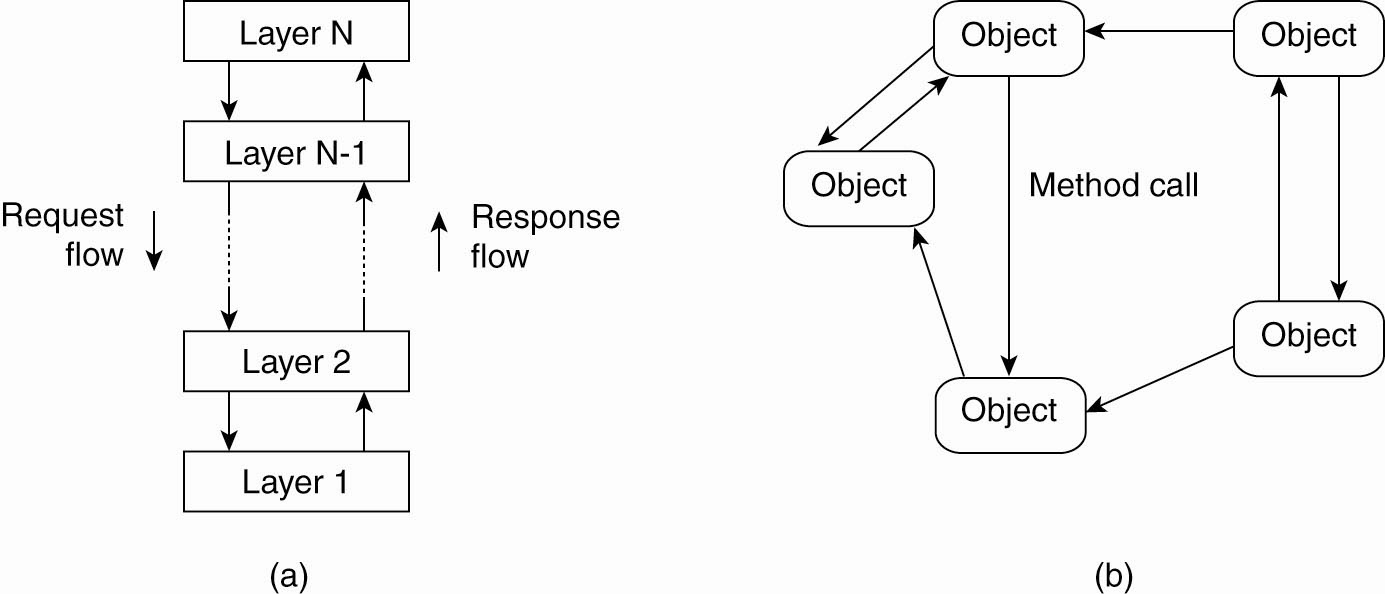
\includegraphics[width=0.5\textwidth]{images/layered}
      \caption{The layered (a) and object-based (b) architectural style}
      \label{layered}
    \end{figure}
  \item \textbf{Object based (figure~\ref{layered})}\\
    Here, objects can call other objects.
  \item \textbf{Event based (figure~\ref{event-based})}\\
    Often used as a publish-subscribe (pub-sub) architecture.
    \begin{figure}[H]
      \centering
      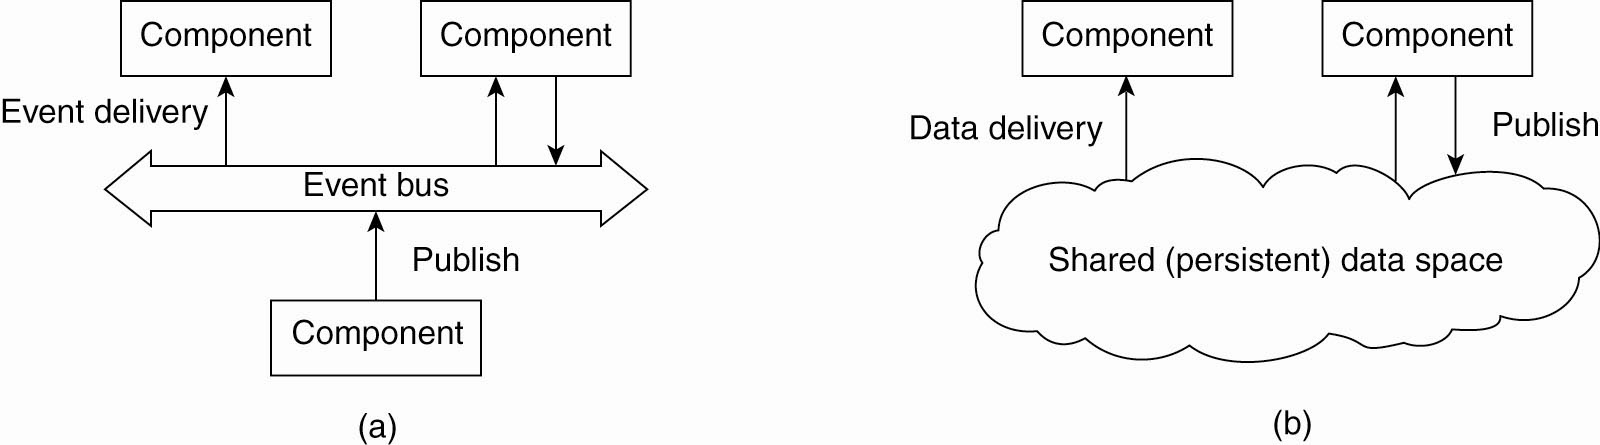
\includegraphics[width=0.5\textwidth]{images/event-based}
      \caption{The event-based (a) and shared-dataspace(b) architectural style}
      \label{event-based}
    \end{figure}
  \item \textbf{Shared dataspace (figure~\ref{event-based})}\\
    % TODO: Defo describe more
    \dots
\end{description}

\textbf{Middleware} is used to abstract away the complexity of dealing with
networks and their issues. Good middleware can effectively hide heterogeneity of
the underlying platforms (e.g. Windows x86 computers talking to Linux ARM
machines). The \textbf{end-to-end} argument reminds us of the limits of
middleware; and states that the functions specific to each application should
reside at the endpoints of the network, not the intermediary hosts. This means
that though middleware can provide generic functions for you to use, you still
have to apply these functions in your application in order to do something
useful.

\subsubsection{Client-Server model}

In this model, many clients will invoke functions on a remote server. Servers
(despite there being few of them) act as the slave, since they are passive and
wait for requests to come. Clients are masters, since they are active, and send
requests to servers. Servers can be stateful or stateless.

Client server architectures, by nature, are asymmetrical. As a result of this,
they often scale poorly, since the server load will increase proportional to the
number of clients. Of course, you can use multiple servers to spread the load on
any one server (horizontal scaling, done using proxies), and put caches between
the client and the server to server common and easy requests.

Another way to reduce the load on servers is to use `mobile code'. Popularised
by Java, this is when code is downloaded to a client from the server, and the
client executes the application locally. This reduces server load, and makes the
app responsive on the user's computer.

The opposite side to this, is having thin clients, who rely on the server to do
all of the heavy lifting for them (e.g. a very simple web browser like Lynx).

\subsubsection{Peer to Peer (P2P) model}

Here, all nodes in the network are the same, and they all talk to eachother.
These networks have no central point of coordination (or failure), which
provides resilience, yet at the same time, complexity.

Though P2P architectures scale well (since they are truly `distributed'), it is
hard to find, coordinate and use resources over the network because of a lack of
any central organisation.

% TODO: Checksums